\chapter{Noise in datasets}
\label{ch:noiseindatasets}\index{noise in datasets|(}

As defined by \citet{hickey1996noise}, noise is anything that distorts the relationship between the describing attributes and the class.  Broadly speaking there are two types of noise: attribute (or feature) noise\index{noise in datasets!attribute noise} and class (or label) noise\index{noise in datasets!class noise} \citep{garcia2013, frenay2014classification}. In attribute noise, errors in one or more of the attributes that describe the class distort the true representation of the data.  Class noise on the other hand, is the mislabelling of instances in a dataset.  Missing observations can exist in both attributes and class, and are also considered as noise \citep{zhu2004class}.

The example dataset in Table~\ref{tab:noise_example} shows the various forms of noise. Instances \textit{5} and \textit{6} exhibit attribute noise, with instance \textit{5} having a missing value for attribute \textit{x\textsubscript{1}}, and instance \textit{6} having attribute \textit{x\textsubscript{2}} erroneously marked as \textit{c}. Instances \textit{1}, \textit{2}, \textit{4} and \textit{7} exhibit class noise.  Instance \textit{1} was mislabelled as \textit{0}, which should read \textit{1}.  Instances \textit{2} and \textit{4} are contradicting instances, implying that either one was mislabelled or the attribute readings were interpreted differently. Instance \textit{7} has a missing label.

\begin{margintable}
  \centering
  \fontfamily{ppl}\selectfont
  \begin{tabular}{cccc}
    \toprule
        \textit{\#} & \textit{x\textsubscript{1}} & \textit{x\textsubscript{2}} & \textit{Y} \\
    \midrule
    1 & a & d & \textcolor{red}{0} \\
    2 & a & c & \textcolor{red}{1} \\
    3 & b & c & 1 \\
    4 & a & c & \textcolor{red}{0} \\
    5 & \textcolor{red}{-} & d & 0 \\
    6 & b & \textcolor{red}{c} & 1 \\
    7 & b & d & \textcolor{red}{-} \\
    \bottomrule
  \end{tabular}
  \caption{A sample from a noisy dataset. \textit{Note: Noise is marked in red for ease of demonstration.}}
  \label{tab:noise_example}
\end{margintable}


Attribute noise is normally introduced through errors in the data collection or data processing stages, but also by corruption whilst the data are stored or transported \citep{garcia2013}.  Class noise on the other hand can be introduced through \citep{frenay2014classification}:
\begin{itemize}[-]
	\setlength{\itemsep}{0pt}
  	\setlength{\parskip}{0pt}
  	\setlength{\parsep}{0pt}
	\item insufficient information when labelling the instances;
	\item expert labelling errors; 
	\item subjectivity of the classes (for example in the case of medical diagnosis where experts can classify differently);
	\item encoding and communication problems; and
	\item using a cheap labelling method (such as non-expert or automated approaches). 
\end{itemize}

Unfortunately, noise is very common since reliable, noise free data are expensive and time consuming to obtain \citep{frenay2014classification}. The typical error rate in a dataset is 5\%. \citep{zhu2004class}. 


\section{Effects of noise}\label{sec:noise_effects}\index{noise in datasets!effects}

When learning a concept, algorithms assume and expect a correct and perfectly labelled dataset \citep{frenay2014comprehensive}.  Primarily, the noise in the training set reduces the predictive ability of the inferred model \citep{garcia2013, frenay2014comprehensive, frenay2014classification}. This can be seen in Figure~\ref{fig:noise_models} that shows the effect of noise on the classification accuracy of various classifiers.

\begin{figure}
  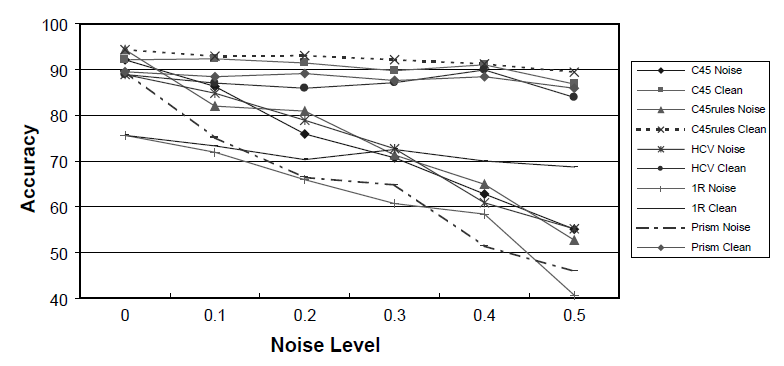
\includegraphics{graphics/noise_in_datasets/noise_models.png}
  \caption{A graph showing the effect of noise on the classification accuracy of various classifiers. Each model was trained on a noisy dataset and on a manually cleaned dataset. These are represented as \textit{XXX Noise} and \textit{XXX Clean} respectively, where \textit{XXX} denotes the classifier in question \citep{zhu2004class}.}
  \label{fig:noise_models}
\end{figure}

The extent of the damage caused by noise depends on various factors.  Class noise\index{noise in datasets!class noise} has been found to be more harmful than attribute noise\index{noise in datasets!attribute noise} \citep{zhu2004class}.  The reason for this is that whilst an attribute shares the predictive capability with other attributes, there is only one label and errors confuse the learning algorithm  \citep{zhu2004class}. 

\citet{zhu2004class} also found that not all attributes are equal in predicting the class and noise in the more important features are more damaging than others. The authors found that the higher the correlation between attribute and class the greater the impact of noise in the attribute.

Learning from a noisy dataset requires a larger training set \citep{frenay2014comprehensive, frenay2014classification} and is usually lengthier \citep{garcia2013}. Another cost of noise is the higher complexity of the inferred model \citep{garcia2013, frenay2014comprehensive, frenay2014classification}.

\section{Dealing with noise}\label{sec:noise_dealing}

To improve the performance of the inferred model, the effect of noise must be minimised \citep{zhu2004class}. There are various ways addressed in literature by which one can minimise such effects, which can be broadly classified into two categories: (i) improving the quality of the dataset (i.e. cleansing noise); and (ii) building models that are robust to noise.

\subsection{Cleansing noise}\label{sec:noise_cleansing}\index{noise in datasets!cleansing}

Noise is usually identified by a domain expert since automatic noise identification is difficult \citep{garcia2013}.  However, a domain expert is not always available and manual identification of noise is a lengthy process, therefore automated noise identification techniques are needed that either correct the noisy data or eliminate it. 

One cannot identify noise without making assumptions \citep{frenay2014classification}. Techniques that filter out noise remove instances that appear mislabelled or that disproportionately increase the model complexity \citep{frenay2014comprehensive}.  In some cases a classifier (noise filter) is trained to identify noisy instances. Other techniques aim at correcting errors or imputing missing values \citep{zhu2004class}.

For class noise\index{noise in datasets!class noise}, filtering out instances that appear noisy was found to improve results, but in the case of attribute noise\index{noise in datasets!attribute noise}, removing an instance for a noisy (including missing) attribute would not make sense, especially since other attributes may contain information that is useful for learning \citep{zhu2004class}. Instead, correcting or imputing the values was found to achieve better results. Techniques that deal with class noise include \textit{ensemble filters}, \textit{cross-validated committees filters} and \textit{iterative-partitioning filters} \citep{garcia2015data}.

Ensemble filters\index{noise in datasets!ensemble filters} aim to identify and remove mislabelled instances in the pre-processing phase \citep{garcia2015data, brodley1999identifying}. The filter consists of an ensemble of \textit{m} different classifiers (for example a decision tree, a 1-NN and an SVM) that are trained on the training data to act as noise filters. The training data is split into \textit{n} parts and for each of the \textit{m} classifiers, \textit{n} different algorithms are trained. Each algorithm classifies one of the \textit{n} subsets after being trained on the remaining \textit{n-1} subsets. If the predicted class does not match the true class, the element is marked as potentially noisy. The results of each of the \textit{m} classifiers are then compared and a consensus whether an element is noisy is obtained through a voting scheme.  Elements deemed noisy are removed from the training data.

Cross-validated committees filters\index{noise in datasets!cross-validated committees filters} use an approach very similar to that of ensemble filters except that the ensemble is made up only of decision trees \citep{garcia2015data, verbaeten2003ensemble}. It uses k-fold cross-validation to split the training data and train the base classifiers. Once again the noisy elements are identified through a voting scheme and eliminated.

Iterative-partitioning filters\index{noise in datasets!iterative-partitioning filters} are used for cleaning large datasets \citep{garcia2015data}. The training data is partitioned into manageable parts and cleansed in iterations until a stopping criterion is met. The stopping criterion is normally the percentage of noise that is tolerated.

\begin{figure}
  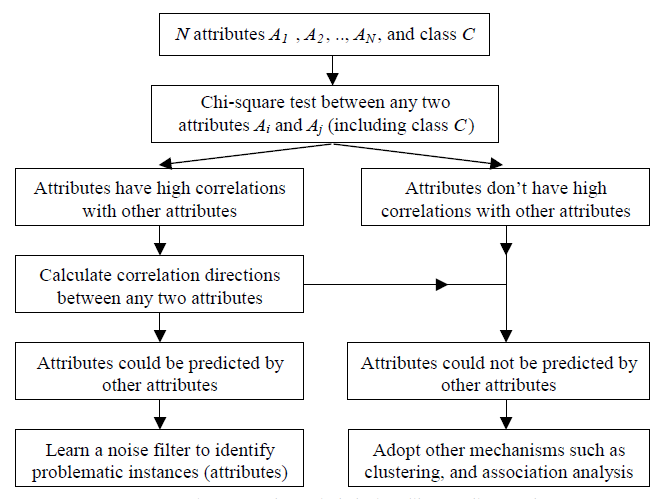
\includegraphics{graphics/noise_in_datasets/noise_imputation.png}
  \caption{The approach adopted by \citet{zhu2004class} to filter and correct attribute noise.}
  \label{fig:noise_imputation}
\end{figure}

Figure~\ref{fig:noise_imputation} depicts the approach taken by \citet{zhu2004class} to correct attribute noise\index{noise in datasets!attribute noise}, where for each attribute a strong correlation with other attributes is sought upon which noisy instances can be predicted (through a learning model) and corrected.  If a correlation is not found, corrections are based on other methods such as \textit{clustering} or \textit{k-nearest neighbour}.

The choice of noise filtering method should be based on the task at hand \citep{frenay2014classification}. The effectiveness of the noise filter should be evaluated on a dataset that is degraded with artificial noise\index{noise in datasets!artificial}.  The filtering precision can then be calculated through the number of correct instances that are filtered\index{noise in datasets!Type I errors} (\textit{Type I errors} - Equation~\ref{eq:noise_type1}) and the number of incorrect instances that are not filtered (\textit{Type II errors} - Equation~\ref{eq:noise_type2})\index{noise in datasets!Type II errors}.  These are calculated as follows: 

\begin{equation}\label{eq:noise_type1}
	ER\textsubscript{1} = \frac{\textnormal{\# of correctly labelled instances which are removed}}{\textnormal{\# of correctly labelled instances}}
\end{equation}

\begin{equation}\label{eq:noise_type2}
	ER\textsubscript{2} = \frac{\textnormal{\# of mislabelled instances which are not removed}}{\textnormal{\# of mislabelled instances}}
\end{equation}

Consequently, the \textit{Noise Elimination Precision} (NER)\index{noise in datasets!Noise Elimination Precision} can be calculated through Equation~\ref{eq:noise_ner} \citep{frenay2014classification}.

\begin{equation}\label{eq:noise_ner}
	NER = \frac{\textnormal{\# of mislabelled instances which are removed}}{\textnormal{\# of removed instances}}
\end{equation}

\subsection{Noise robust models}\label{sec:noise_robust_models}\index{noise in datasets!noise robust models}

No learning algorithm is immune to noise but some algorithms perform better than others in the presence of noise \citep{frenay2014comprehensive}.  \citet{kalapanidas2003machine} studied the noise sensitivity of ten different machine learning algorithms against various levels of artificially induced noise.  The results show that classifiers are much more noise tolerant than regressors.  The \textit{linear regression} algorithm proved to be the regressor least sensitive to noise, whilst the \textit{decision table classifier} proved to be the best performer overall.  A similar study \citep{nettleton2010study} found the \textit{na\"ive bayes} algorithm to be the most robust to noise.

\index{noise in datasets|)}